% Appendix for the ICLR 2027 submission.
% Included from main.tex after \appendix. Every number here resolves to a macro
% in numbers.tex or to a table generated from results/.

\clearpage
\section{Notation}
\label{app:notation}

\begin{center}
\small
\begin{tabular}{ll}
\toprule
Symbol & Meaning \\
\midrule
$I_t = (P_t, c_t, b_t, N_t, A_t)$ & edition $t$: projects, costs, budget, voters, ballots \\
$A_t(i) \subseteq P_t$ & the approval ballot of voter $i$ \\
$A_t(p) \subseteq N_t$ & the approvers of project $p$ \\
$N_t^{\mathrm{cov}}\subseteq N_t$ & voters with the demographics needed for the group ledger \\
$G$ & the group partition (age $\times$ sex cells the ballots record) \\
$g_t$ & covered members of group $g$ among edition-$t$ voters \\
$W_t \subseteq P_t$ & the funded set, $c_t(W_t) \le b_t$ \\
$u_t(g)$ & money attributed to $g$ (Definition~\ref{def:csd}) \\
$e_t(g)$ & entitlement of $g$, its share of money spent \\
$\csd_T(g)$ & cumulative share deficit of $g$ after $T$ editions \\
$\mathcal{H}_{t-1}$ & history available to a policy entering edition $t$ \\
$\beta_i$ & endowment of voter $i$; uniform $\beta_i = b_t/|N_t|$ is \MES \\
$w \in \mathbb{R}^{6}$ & endowment-family weights \\
$v \in \mathbb{R}^{5}$ & outcome-family weights \\
$\rho$ & Equal Shares price level at which a project is bought \\
$\kappa$ & largest endowment multiple, $\max_i \beta_i |N_t| / b_t$ \\
$\tau, \mu$ & soft welfare target and its penalty weight \\
$\lambda$ & rollover intensity of \RES \\
\bottomrule
\end{tabular}
\end{center}

\section{Corpus and splits}
\label{app:corpus}

\paragraph{Construction.}
We build the fitting corpus from the frozen Pabulib snapshot
\citep{stolicki2020pabulib}. We keep nonempty approval elections with recorded
winners, at most $300{,}000$ voters, and demographic data on at least half
of the ballots. We then group elections by (city, district). A group qualifies
as a \emph{series} if its longest consecutive run contains at least three
editions. The corpus contains
\NumSeriesTotal{} series and \PrimaryElectionN{} elections, comprising
\PrimaryBallotN{} ballots and \PrimaryProjectN{} projects from
\PrimaryYearLo--\PrimaryYearHi. We exclude the Warsaw citywide contest and a
Wawer subunit because both aggregate ballots that already appear in the
district series.

\paragraph{Fitting corpus versus available corpus.}
We fit the headline Warsaw weights only on the primary corpus above. Applying
the same filter to the complete public repository admits many additional
series, mostly outside Warsaw, including histories in Gdynia and \L{}\'od\'z
that are long enough for the temporal protocol. An earlier version used an
incomplete local download and incorrectly attributed its limited coverage to
the public data. We corrected the download without refitting the headline
weights. The locked projected-support study uses separate pooled-temporal
fits trained on pre-2023 histories from Gdynia, Warsaw, and \L{}\'od\'z. For
the post-hoc native-approval replay, we use the frozen Warsaw headline fit.
We report no fit on the complete corpus.

\paragraph{Corrected-result lineage.}
The primary Warsaw results come from a saved corrected replay with duplicate
project tokens removed within each ballot and a deterministic project order.
Canonicalization removes one repeated approval token in Wola 2021; no ballot
is removed. The corrected corpus contains 6,577,175 approval tokens across
\PrimaryBallotN{} ballots. We retain the original artifacts and authenticate
the corrected fit and evaluation records separately. Because the original
results had already been inspected, the corrected Warsaw and first multi-city
analyses are post-hoc replays, not new untouched holdout tests. The first
multi-city decision remains \emph{falsified}. The projected-support external
study and the native-approval replay retain their separate recorded lineages.
The manuscript reconstruction uses saved estimates and intervals; it does not
rerun fitting or statistical tests.

\paragraph{Missing demographics.}
Every ballot contributes to the \emph{allocation}. When age or sex is missing,
the approvals still affect funding, but the ballot cannot enter the cohort
ledger because we cannot assign it to a group. Project scores therefore count
all ballots, while the fairness ledger counts only covered ballots. Confusing
these counts caused the defect described in Appendix~\ref{app:containment}.
The filter requires demographics on half of an election's ballots. We do not
model why fields are missing. If coverage depends on age or sex, for example
through the voting channel, the ledger represents a nonrandom subsample, and
that selection affects every deficit, entitlement, and $\csd$ value. We do
not test this missingness assumption.

\paragraph{Splits.}
The temporal split fits on editions through 2022 and evaluates on 2023--2025:
\SplitTrainEditions{} training editions and \SplitTestEditions{} held-out
editions across \EvalSeriesN{} series. The \L{}\'od\'z citywide contest enters
the fitting corpus only in 2023 and thus has no training editions. We exclude
that series from the temporal split and use it for the no-refit city-out replay
in Section~\ref{sec:transfer}. The district series available in the complete
repository are held out entirely for Appendix~\ref{app:external}. We use no
\L{}\'od\'z data to fit the primary temporal policies. Repeated analysis of
the citywide series limits its role to a descriptive transfer case rather than
external validation.

A separate five-fold disjoint-series check uses the complete history of every
series. We hold \L{}\'od\'z out in one fold and include it in training in the
other four. This check evaluates disjoint series, so it tests neither temporal
nor Warsaw-to-\L{}\'od\'z transfer. We save each split to disk and reload it
to keep the boundaries fixed across runs.

Here, held-out editions are excluded from fitting the shared weight vector.
Allocation still uses the edition-$t$ ballots, project costs, and budget once
they are available. The recorded winner set is never a policy feature. Each
counterfactual policy replays a series in order and updates
$\mathcal{H}_{t}$ using only its own selected outcome after scoring edition $t$.

\section{Feature definitions}
\label{app:features}

Every feature is dimensionless. Setting $w=0$ in the endowment parametrization
recovers \MES. In the outcome family, $v=e_1$ and $v=e_2$ recover the two
baselines, while the zero vector does not. Let $n = |N_t|$, $b = b_t$, and
write $\bar{\ell}$ for the mean ballot length over covered voters.

\paragraph{Endowment family.}
For group $g$ with carried deficit $D_{t-1}(g) = \sum_{\tau<t}(e_\tau(g) - u_\tau(g))$
and carried entitlement $E_{t-1}(g) = \sum_{\tau<t} e_\tau(g)$:
\begin{align*}
f_1(g) &= \frac{\max(0, D_{t-1}(g))}{|g_t| \cdot (b/n)}
  &&\text{deficit per capita, in units of the base endowment}\\
f_2(g) &= \mathrm{clip}\!\left(\frac{D_{t-1}(g)}{E_{t-1}(g)},\, -1,\, 1\right)
  &&\text{signed deficit as a fraction of entitlement owed}\\
f_3(g) &= \frac{|g_t|}{n_{\mathrm{cov}}} - \frac{1}{|G|}
  &&\text{size relative to an equal split}\\
f_4(g) &= \frac{\bar{\ell}_g}{\bar{\ell}} - 1
  &&\text{ballot length relative to the electorate}\\
f_5(g) &= \frac{\bar{c}_g}{\bar{c}} - 1
  &&\text{mean cost per approval, relative}\\
f_6(g) &= \cos\!\big(\phi_g, \phi_{\mathrm{all}}\big) - \overline{\cos}
  &&\text{approval-profile overlap, mean-centred over groups}
\end{align*}
Here $\phi_g$ is the vector of per-project approval frequencies within $g$.
History enters only through $f_1$ and $f_2$. A voter without recorded
demographics receives raw endowment $b/n$. For a covered voter,
$w = \lambda e_1$ gives raw endowment
$b/n + \lambda \max(0, D_{t-1}(g))/|g_t|$. The common budget normalization then
recovers \RES{} exactly.

\paragraph{Outcome family.}
For project $p$ with $\mathrm{sh}(p) = |A_t(p)|/n$ counted over \emph{all}
ballots and $\mathrm{cs}(p) = c_t(p)/b$:
\begin{align*}
\varphi_1(p) &= \mathrm{sh}(p) &&\text{approval share} \\
\varphi_2(p) &= \frac{\mathrm{sh}(p)/\mathrm{cs}(p)}{\max_q \mathrm{sh}(q)/\mathrm{cs}(q)}
  &&\text{approvals per unit cost, normalized to } [0,1] \\
\varphi_3(p) &= \mathrm{cs}(p) &&\text{cost share} \\
\varphi_4(p) &= \sum_{g} \hat{w}_g \cdot
  \frac{n_{t,g}(p)}{n_t^{\mathrm{cov}}(p)}
  &&\text{support drawn from lagging groups} \\
\varphi_5(p) &= \sqrt{\frac{\sum_g \big(s_g(p) - 1/|G|\big)^2}{1 - 1/|G|}}
  &&\text{concentration of support across groups}
\end{align*}
If at least one group has a positive deficit, the weights satisfy
$\hat{w}_g \propto \max(0, D_{t-1}(g))$ and sum to one. Otherwise, all weights
are zero. The term $s_g(p)$ is the
share of $p$'s covered approvers in $g$. Only $\varphi_4$ uses history. A ratio
over covered approvers is set to zero when the project has no covered approver.
Setting $v=e_1$ recovers greedy approval count, and $v=e_2$ recovers greedy
approvals per unit cost.

The supporter-composition diagnostic in Section~\ref{sec:theory} uses
$q_{t,g}(p)$ for group $g$'s share among the demographically covered approvers
of project $p$, and $s_{t,g}=|g_t|/\sum_h |h_t|$ for its share among covered
voters. We report
\[
\operatorname{TV}_t(p)=\frac{1}{2}\sum_g
  \left|q_{t,g}(p)-s_{t,g}\right|,
\]
as a raw-cost-weighted average over funded projects. We compute this quantity
only on held-out editions after replaying each policy's training prefix.
The optimizer uses this descriptive measure neither as a feature nor as an
objective.

\section{Mechanism implementation}
\label{app:mechanism}

\begin{algorithm}[ht]
\caption{Equal Shares with general endowments, and completion}
\label{alg:mes}
\begin{algorithmic}[1]
\Require instance $(P, c, b, N, A)$, endowments $\beta \ge 0$
\State $W \gets \emptyset$;\; $\mathcal{A} \gets \{p : A(p) \neq \emptyset,\, c(p) > 0\}$
\While{$\mathcal{A} \neq \emptyset$}
  \ForAll{$p \in \mathcal{A}$}
    \If{$\sum_{i \in A(p)} \beta_i < c(p)$} \State $\mathcal{A} \gets \mathcal{A} \setminus \{p\}$ \Comment{never affordable; endowments only shrink}
    \Else \State $\rho_p \gets \min\{\rho : \sum_{i \in A(p)} \min(\beta_i, \rho) \ge c(p)\}$
    \EndIf
  \EndFor
  \State \textbf{if} $\mathcal{A} = \emptyset$ \textbf{then break}
  \State $p^\star \gets \arg\min_{p \in \mathcal{A}} \rho_p$ \Comment{ties by ascending cost, then id}
  \State $\beta_i \gets \beta_i - \min(\beta_i, \rho_{p^\star})$ for $i \in A(p^\star)$
  \State $W \gets W \cup \{p^\star\}$;\; $\mathcal{A} \gets \mathcal{A} \setminus \{p^\star\}$
\EndWhile
\State \Comment{completion: Equal Shares is not exhaustive, so spend the remainder}
\State $r \gets b - c(W)$
\ForAll{$p \notin W$ with $A(p)\neq\emptyset$ in descending $|A(p)|$,
  ties by ascending $c(p)$, then id}
  \If{$c(p) \le r$} \State $W \gets W \cup \{p\}$;\; $r \gets r - c(p)$ \EndIf
\EndFor
\State \Return $W$
\end{algorithmic}
\end{algorithm}

Completion spends the remaining budget by approval count and falls outside the
payment rule. It accounts for the nonzero uniform Equal Shares value in
Table~\ref{tab:infeasible}; the learned-endowment value uses the same uniform
reference floor, not the learned cap. We find $\rho_p$ in one pass over the
sorted approver endowments. The absolute tolerance is $10^{-9}$ for aggregate
affordability and $10^{-12}$ for water-filling breakpoints.

\begin{algorithm}[ht]
\caption{Outcome family, with an optional support floor}
\label{alg:outcome}
\begin{algorithmic}[1]
\Require instance, weights $v$, optional $\kappa$
\State $E \gets \{p : A(p) \neq \emptyset\}$
\If{$\kappa$ given} \State $E \gets \{p \in E : |A(p)|/n \ \ge\ c(p)/(\kappa b)\}$ \EndIf
\State $W \gets \emptyset$;\; $r \gets b$
\ForAll{$p \in E$ in descending $v^{\top}\varphi(p)$, ties by ascending
  $c(p)$, then id}
  \If{$c(p) \le r$} \State $W \gets W \cup \{p\}$;\; $r \gets r - c(p)$ \EndIf
\EndFor
\State \Return $W$
\end{algorithmic}
\end{algorithm}

\section{Optimization}
\label{app:optim}

We fit both arms with the same self-contained CMA-ES implementation. It uses
\OptimizerLines{} lines of NumPy and runs without a GPU or dependencies on
SciPy, cma, or PyTorch.

\begin{table}[ht]
\centering\small
\begin{tabular}{lcc}
\toprule
 & Endowment arm & Outcome arm \\
\midrule
Search dimension & 6 & 5 \\
Population $\lambda = 4 + \lfloor 3\ln d\rfloor$ & 9 & 8 \\
Parents $\mu = \lfloor \lambda/2 \rfloor$ & 4 & 4 \\
Initial step $\sigma_0$ & 0.4 & 0.4 \\
Generations & 30 (headline); 25 (frontier/stability) & 25 \\
Objective evaluations & 271 headline; 225 frontier; 226 stability & 200 per target \\
Weight box & $[-10, 10]$ & $[-10, 10]$ \\
Penalty weight $\mu$ & 0 headline; 0/2.0 frontier & 0/2.0 frontier \\
Seeds & 42, 1, 2 & 42, 1, 2, 3 \\
Corrected-run wall clock & Not recorded & Not recorded \\
\bottomrule
\end{tabular}
\caption{Optimizer settings. In Section~\ref{sec:ablation}, ``same optimization
budget'' means 25 generations with population 8, as in the frontier fits used
for comparison. The original fits used \computehardware, without a GPU.
The corrected fit artifacts do not record elapsed times, so we do not report
corrected-run wall-clock ranges. Endowment evaluation replays iterative Equal
Shares; the outcome arm uses a greedy pass.}
\end{table}

The headline endowment fit and its two additional seeds use different numbers
of generations. Their range gives an informal check of optimizer stability,
with no estimate of variance under matched optimization budgets.

Each of the five primary disjoint-series fits uses 25 generations and the
coefficient box $[-10,10]$. All five reach the boundary. We therefore ran a
matched post hoc set with box $[-40,40]$ and separate artifact tags, but four
of the wider fits also reach their boundary. Table~\ref{tab:district-bound}
compares held-out outcomes. These results support neither coefficient
interpretation nor a claim of independent replication.

We leave the features unstandardized. Election-level ratios are dimensionless,
and the two history features retain their longitudinal scale. No fit uses a
restart. We initialize the means at the hand-designed references \RES$(1)$
for endowments and greedy approvals-per-cost for outcomes. Because CMA-ES need
not return its initial mean as a candidate, we replay and report every
baseline separately.

\paragraph{Why distinct soft welfare targets can return identical policies.}
The penalty is $\mu \max(0, \tau - \text{ratio})$. When the unconstrained
optimum exceeds $\tau$, it incurs no penalty and remains optimal. If $\tau$
exceeds every attainable welfare ratio, each candidate incurs
$\mu(\tau - \text{ratio})$. Increasing $\tau$ then adds the same constant to
every objective value, leaving the minimizer unchanged. The trade-off changes
only in the intermediate regime. This formulation explains the identical rows
in Table~\ref{tab:endowfrontier} without implying a failed search.

We use $\tau=1$ as the headline outcome-arm operating point because its
training target equals \MES{} approval-count welfare. Neither this choice nor
the penalty weight $\mu=2$ was preregistered. Table~\ref{tab:endowfrontier}
reports the full tested target grid. The headline selection remains
exploratory.

\section{Containment verification}
\label{app:containment}

\begin{table}[ht]
\centering\small
\begin{tabular}{lccc}
\toprule
Identity & Scope & Tolerance & Result \\
\midrule
$w = \mathbf{0} \Rightarrow \MES$ & \NumSeriesTotal{} series & exact & max $|\Delta| = 0$ \\
$w = \lambda e_1 \Rightarrow \RES(\lambda)$, 5 values & \NumSeriesTotal{} series & exact & max $|\Delta| = 0$ \\
$v = e_1 \Rightarrow$ greedy-by-count & \PrimaryElectionN{} elections & set equality & \PrimaryElectionN{}/\PrimaryElectionN{} \\
$v = e_2 \Rightarrow$ greedy-by-cost & \PrimaryElectionN{} elections & set equality & \PrimaryElectionN{}/\PrimaryElectionN{} \\
environment vs.\ frozen replay & \NumSeriesTotal{} series, 3 rules & $5\times10^{-4}$ & \NumSeriesTotal{}/\NumSeriesTotal{} \\
\bottomrule
\end{tabular}
\end{table}

The first run failed the third identity on 4 of \PrimaryElectionN{} elections.
The learned score counted approvals only on demographically covered ballots,
while the deployed rule counted every ballot. These counts agree when coverage
is complete, but partial coverage can change the project order. We corrected
the implementation by separating allocation counts from ledger counts
(Appendix~\ref{app:corpus}). The containment test found the defect, which code
review had not detected. Without that check, the wrong counts could have
produced plausible results.

\section{Proof of Proposition~\ref{prop:support}}
\label{app:proof}

\begin{proof}
Let $W_{\mathrm{pay}}$ be the outcome of Algorithm~\ref{alg:mes} before
completion, and let $p \in W_{\mathrm{pay}}$ be bought at price level $\rho$.
By the purchase rule, $p$ enters $W_{\mathrm{pay}}$
only when its approvers can cover its cost at that level:
\[
\sum_{i \in A(p)} \min(\beta_i^{(p)}, \rho) \;\ge\; c(p),
\]
where $\beta^{(p)}$ are the endowments remaining when $p$ is bought. Endowments
are non-increasing along the run, since each purchase only subtracts, so
$\beta_i^{(p)} \le \beta_i$ for the initial vector $\beta$. Also
$\min(x, \rho) \le x$. Chaining these,
\[
c(p) \;\le\; \sum_{i \in A(p)} \min(\beta_i^{(p)}, \rho)
      \;\le\; \sum_{i \in A(p)} \beta_i^{(p)}
      \;\le\; \sum_{i \in A(p)} \beta_i .
\]
Now suppose $\beta_i \le \kappa\, b/|N|$ for every $i$. Then
$\sum_{i \in A(p)} \beta_i \le |A(p)| \cdot \kappa b / |N|$, and combining with
the display above gives $c(p) \le |A(p)| \kappa b / |N|$, i.e.
$|A(p)|/|N| \ge c(p)/(\kappa b)$, which is the claim.
\end{proof}

The bound is attained when every approver of $p$ still holds exactly
$\kappa b/|N|$ and spends the full amount on $p$, as can happen when none has
paid for an earlier winner. Otherwise the bound is generally slack. Under the
stated cap, the proposition restricts payment-phase purchases but does not
determine a fitted policy's choices. Section~\ref{sec:identification} tests that
region constraint separately and finds that it does not reproduce the
mechanism.

\section{Representative support: proof and executable check}
\label{app:degeneracy}

\begin{proof}[Proof of Proposition~\ref{prop:representative}]
For a fixed group $g$, Definition~\ref{def:csd} and the definitions of
$q_{t,g}(p)$ and $E_g$ give the following, where
$\omega_{t,p,g}=c_t(p)s_{t,g}/E_g$ and
$r_{t,p,g}=q_{t,g}(p)/s_{t,g}$:
\begin{align*}
\csd_T(g)
&= 1-\frac{\sum_t\sum_{p\in W_t}c_t(p)q_{t,g}(p)}{E_g} \\
&= 1-\sum_t\sum_{p\in W_t}
  \frac{c_t(p)s_{t,g}}{E_g}\frac{q_{t,g}(p)}{s_{t,g}}
 = 1-\sum_t\sum_{p\in W_t}\omega_{t,p,g}r_{t,p,g}.
\end{align*}
Because
$\sum_{t,p}\omega_{t,p,g}=\sum_t c_t(W_t)s_{t,g}/E_g=1$,
\[
|\csd_T(g)|
=\left|\sum_{t,p}\omega_{t,p,g}(1-r_{t,p,g})\right|
\leq\sum_{t,p}\omega_{t,p,g}|1-r_{t,p,g}|
\leq\epsilon.
\]

For the construction, let the positive rational group shares be $(s_g)_g$ and choose a
positive integer $m$ such that every $m s_g$ is an integer. Choose a larger
electorate size $n$ with every $n s_g$ integral and $m/n\leq\delta$. Create one
project of cost $b$, approved by exactly $m s_g$ voters from each group, and a
budget-feasible dummy project, also of cost $b$, approved by every other
voter. Fund only the representative project; it exhausts the budget, so the
dummy remains unfunded. Its approver composition is $q_g=s_g$, so the identity
gives $\csd(g)=0$ for every group. Exactly $m$ of $n$ voters approve a funded
project, hence exclusion is $1-m/n\geq1-\delta$.
\end{proof}

The executable construction uses \DegGroups{} equal groups. We keep one
supporter per group and increase the electorate, evaluating each case with the
same \texttt{group\_outcome},
\texttt{cumulative\_share\_deficit}, and \texttt{exclusion\_rate} functions used
in the experiments.

\begin{table}[ht]
\centering\small
\begin{tabular}{rrrr}
\toprule
Voters & Winner supporters & Worst $|\csd|$ & Exclusion \\
\midrule
\DegEightyVoters & \DegSupporters & \DegEightyCSD & \DegEightyExcl \\
\DegTwoHundredVoters & \DegSupporters & \DegTwoHundredCSD & \DegTwoHundredExcl \\
\DegFourHundredVoters & \DegSupporters & \DegFourHundredCSD & \DegFourHundredExcl \\
\DegEightHundredVoters & \DegSupporters & \DegEightHundredCSD & \DegEightHundredExcl \\
\bottomrule
\end{tabular}
\caption{Representative-support construction from
\texttt{iclr\_degeneracy.py}. CSD remains exactly zero in the production ledger
as exclusion approaches one. This construction tests the metric's limits. It
is neither a fitted result nor a candidate policy.}
\label{tab:degeneracy}
\end{table}

\begin{figure}[tb]
\centering
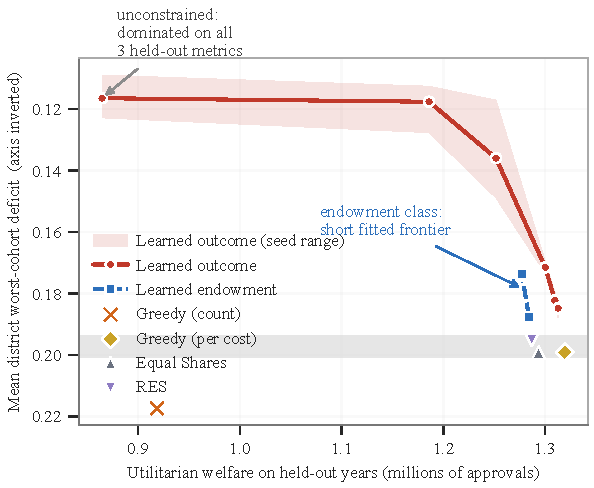
\includegraphics[width=0.72\textwidth]{fig_frontier.pdf}
\caption{Held-out fairness--welfare results for the fitted policy classes. The
grey band covers four hand-designed rules: greedy approvals/cost, \MES{}, and
\RES{}$(\lambda{=}0.5,1.0)$. Its width is \HandBandWidth. Both learned classes
extend beyond the band. Direct scores span \RangeOutcomeWidth{} (red, with
variation across \NumSeeds{} seeds), while learned endowments span
\RangeEndowWidth{} (blue). The classes learn different objects from different
features, so this comparison cannot identify the causal effect of the payment
rule. Mild regularization improves both fairness and welfare over the
unpenalized direct-score point.}
\label{fig:frontier}
\end{figure}

\section{Statistical methodology}
\label{app:stats}

We use the \emph{series} as the inferential unit. Editions within a district
share a project pool and electorate, and the districts themselves belong to
one city. The intervals describe dispersion across districts in this corpus.
They cannot remove common-city shocks or support city-level population
inference. For each policy contrast, we first calculate the difference in
held-out worst-group $\csd$ within each series, then take an equally weighted
mean across series. The reported $2.5$--$97.5$ paired percentile-bootstrap
interval uses $10{,}000$ resamples of these series pairs.

The exact paired test enumerates all $2^{\EvalSeriesN}$ sign assignments of the
series differences under the null. It reports the two-sided fraction whose
absolute mean is at least as large as the absolute observed mean. The test assumes
sign-exchangeable paired differences under the null and treats neither
elections nor voters as independent replicates. We display values below $0.001$
as $p<0.001$. A ``win'' is a series with a negative difference. We report wins
alongside the mean because large improvements in a few series can lower that
mean.

In the disjoint-series analysis, the pooled 19-series mean, win count, and
paired bootstrap interval are descriptive because all series in a held-out
fold share one fitted map. As a sensitivity check, we average the paired
effects within each fold and enumerate all $2^5$ sign assignments of the five
fold means. The fold-block $p$-value has a minimum two-sided resolution of
$0.0625$. These five fits use overlapping training sets and cannot count as
independent replications. This analysis also uses each series' complete
history, so it tests neither temporal nor cross-city transfer.

We apply Holm--Bonferroni correction to the \WarsawHolmFamilyN{} focal held-out
Warsaw comparisons reported in the main text: direct scoring against \MES{},
learned endowments against \MES{}, and the senior tilt against \MES{}. The full
welfare-target grid, closest-prior comparison, matched-target check,
allocation-kernel intervention, and three group partitions remain secondary
exploratory analyses and are unadjusted unless a separate protocol states
otherwise. The partition analyses re-score the same fitted policies, which
makes them dependent. Neither the focal contrasts nor the frozen-score
intervention was preregistered. Adjusting the values controls multiplicity
within this reported family, but the evidence remains exploratory.
In the post-lock audit, the age lookup changes CSD relative to the senior tilt
by \AgeLookupVsSeniorDiff{} (95\% CI \AgeLookupVsSeniorCI, secondary exploratory
$p$~\AgeLookupVsSeniorP, \AgeLookupVsSeniorRecord{} wins/ties/losses).

\section{Extended related work}
\label{app:related}

We expand the comparison in Section~\ref{sec:related} by examining what each
method learns, which mechanism it retains, and how it is evaluated.

\paragraph{Participatory budgeting as a social-choice object.}
Indivisible participatory budgeting extends approval-based committee selection
to projects with costs, bringing many of the same axiomatic questions into a
budgeted setting \citep{aziz2018pbaxioms,talmon2019framework}. Surveys and
systematizations review the available rules
\citep{rey2025survey,los2022systematization}, and handbooks describe their
place in computational social choice
\citep{brandt2016handbook,lackner2022book}. Fairness targets vary.
Prior work studies justified representation
\citep{aziz2015jr,peters2022additive}, the core \citep{fain2016core},
egalitarian or maximin objectives \citep{sreedurga2022maxmin}, equality of
resources \citep{maly2023equality}, and sequential-payment rules such as Equal
Shares and Phragm\'en-style methods
\citep{peters2020welfarism,brill2024phragmen}.

A proportional rule may leave money unspent, so exhaustiveness requires a
separate design choice \citep{papasotiropoulos2025bos}. We evaluate
Algorithm~\ref{alg:mes} with its approval-count completion included. Fair
public decisions outside budgeting \citep{conitzer2017fair} and
sortition-style panel selection \citep{flanigan2021assemblies} also raise group
fairness questions, but they lack the monetary attribution on which CSD is
built.

\paragraph{Fairness across repeated decisions.}
Dynamic social choice studies obligations to voters who lose across a sequence
of decisions \citep{parkes2013dynamic,freeman2017dynamic}. Perpetual voting
formalizes the problem for single-winner sequences
\citep{lackner2020perpetual}, including justified-representation analogues
\citep{bulteau2021perpetual}. Related work extends JR/PJR/EJR to sequences of
unit-cost decisions \citep{elkind2023temporal,elkind2024temporalelections} and
examines verification complexity \citep{elkind2025verifying}, sequential
proportionality \citep{skowron2022public,chandak2026sequential}, adaptive
settings \citep{kraiczy2023adaptive}, and the price of temporal representation
\citep{teh2026price}. Long-term PB for voter types is the closest antecedent
\citep{lackner2021longterm}. These papers mainly analyze axioms and worst
cases, often on synthetic instances. We fit policies within a deployed
mechanism and evaluate them by replaying recorded ballots.

Repeated artificial-currency allocation also uses personalized endowments
\citep{gorokh2016artificial}. There, the endowments parameterize an all-pay
auction for one repeated resource and permit incentive and efficiency
guarantees. We fit endowments from PB data for Equal Shares over combinatorial
public projects. Our evaluation measures group outcomes on recorded ballots
and does not model strategic bids.

Mixed-rule work gives \MES{} a set of projects selected earlier in the same
election. Four hand-designed ``pre-allocation'' methods charge those projects
to voters before rebalancing the remaining budgets \citep{baychkov2026mixed}.
The analysis proves EJR-style guarantees and evaluates within-election
Greedy--\MES{} mixtures on 313 Pabulib instances. Our map uses current group
features and, optionally, prior editions to set endowments before any project
is selected. We compare this payment mechanism with direct winner scores by
measuring held-out fairness, welfare, coverage, and susceptibility to proxy
gaming. We claim neither the first nonuniform \MES{} budgets nor a new EJR
guarantee.

\citet{yang2025komitee} change the virtual-budget population by combining
equal-budget voters with weighted ``value agents'' for deliberatively chosen
impact fields. Participants elicit and co-design the weights for one election.
This changes what the \MES{} ledger represents without fitting endowments from
past allocation outcomes or learning a policy over repeated elections.

\paragraph{Empirical participatory budgeting.}
Pabulib standardizes observed PB instances \citep{stolicki2020pabulib}, following
the PrefLib tradition \citep{mattei2013preflib}. The surrounding infrastructure
includes analysis tools \citep{pabutools2024}, methodological guidance
\citep{faliszewski2023data,boehmer2024guide}, and maps of the instance space
\citep{szufa2020map}. Empirical studies examine ballot formats and elicitation
\citep{fairstein2023realworld,goel2019knapsack,benade2017elicitation}, spatial
fairness across districts \citep{hershkowitz2021districtfair}, interactions in
voter behavior \citep{jain2020interactions,fairstein2024interactions}, and the
utilitarian cost of Equal Shares \citep{baychkov2026utilitarian}. The last
quantity enters the trade-off controlled by our soft welfare target.

Equal Shares is used in practice \citep{equalshares2023}, within a longer policy
history of participatory budgeting \citep{cabannes2004pb}. Existing empirical
designs generally study one election or analyze many elections independently.
We link successive editions of the same district.

\paragraph{Learning allocation objects in participatory budgeting.}
Learning PB aggregation rules predates this paper.
\citet{fairstein2024learningpb} adapt Set Transformers to produce project scores.
They train from example outcomes or explicit objectives, recover or blend
Approval Voting, Chamberlin--Courant, and PAV-like rules, and test on Warsaw
Pabulib elections. At artifact freeze, we found no public implementation of
that model. Reconstructing its architecture and training would require a new
implementation, so we discuss the method without claiming to reproduce it.
\citet{thach2026llmrule} use LLM-guided evolution to generate executable
project-priority programs for utilitarian and Strong-EJR-approximation
objectives. They evaluate more than 600 PB instances and also use the learned
priorities to complete Equal Shares.

Both prior methods learn which projects to select. Our payment-retaining
family learns Equal Shares endowments, which we evaluate with a held-out
longitudinal ledger. We use the direct-outcome family to diagnose objective
gaming through counterfactual replay. We do not propose it for deployment.

Other PB systems learn at different stages.
\citet{adams2026compromises} train voter agents to revise cumulative ballots
while keeping Greedy or Equal Shares fixed. \citet{damle2025llms} prompt
language models to infer preferences and select feasible portfolios. These
methods support voter decisions and reason from language to allocations,
respectively. Neither learns an internal parameter of a recorded allocation
mechanism.

For an executable comparison, we transcribed the two published approval-ballot
scores from \citet{thach2026llmrule} and replayed both without refitting. Count
satisfaction matches our welfare definition, while cost satisfaction does not.
We report both scores to avoid selecting one after observing the results.

\begin{table}[ht]
\centering\small
\begin{tabular}{lccc}
\toprule
Frozen published score & Mean worst-group $\csd$ $\downarrow$ & Welfare $\uparrow$ & Exclusion $\downarrow$ \\
\midrule
LLMRule, cost satisfaction & \LLMRuleCostCSD & \LLMRuleCostWelfare & \LLMRuleCostExcl \\
LLMRule, count satisfaction & \LLMRuleCardCSD & \LLMRuleCardWelfare & \LLMRuleCardExcl \\
\bottomrule
\end{tabular}
\caption{Closest-prior learned rules replayed on the held-out editions using
the published formulas without retraining. The count-satisfaction row supplies
the comparison in Table~\ref{tab:main} because it uses the same approval-count
welfare statistic.}
\label{tab:llmrule}
\end{table}

Beyond PB, deep learning has been used to design auctions, voting rules, and
redistribution mechanisms fitted to human preferences
\citep{duetting2019optimal,mohsin2022learning,koster2022democratic}. We learn
a low-dimensional parameter of an existing proportional payment procedure,
with exact containment checks that recover its hand-designed references. In
the closest mechanism-informed example
outside PB, \citet{maruo2026mechanism} learn missing chore preferences through
differentiable approximations to adjusted winner, round robin, and moving knife.
They learn preference information, while we learn endowments for a fixed
payment procedure.

Contextual resource-allocation metrics can disagree even in the absence of
strategic behavior or optimization failure. Allocation parity and outcome
parity are generally incompatible \citep{jo2023contextual}. We examine a
narrower empirical case. CSD attributes spending by supporter composition, so
direct optimization
over winner sets can match group shares while serving few voters. The tested
payment-retaining class does not reach the same corner under the same objective.
In Section~\ref{sec:identification}, we first decompose the metric and give an
executable construction. We then compare policy classes and test changes to
the allocation kernel with frozen scores.

\paragraph{Properties retained during payment.}
Learning the endowment parametrization preserves budget feasibility and
approver-funded accounting during the payment phase.
Section~\ref{sec:identification} measures the empirical consequence of that
restriction. Nonuniform endowments and greedy completion prevent us from
invoking standard priceability.

\section{Cross-city transfer and breadth stress test}
\label{app:transfer}

\label{sec:transfer}

We fit the primary temporal policies on Warsaw districts through 2022. The
\L\'od\'z citywide contest enters the fitting corpus in 2023, so we exclude
it from that split. The policies below have seen none of its ballots or
projects and no data after 2022. These citywide elections are also an order of
magnitude larger than a Warsaw district election. We replay the frozen
policies without retraining to obtain one descriptive transfer case across
city, time, and scale.

\begin{table}[tb]
\centering
\small
\begin{tabular}{lcc}
\toprule
Rule & Mean worst-group $\csd$ $\downarrow$ & Welfare $\uparrow$ \\
\midrule
Deployed outcome & \TransferHistCSD & \TransferHistWelfare \\
\MES{} & \TransferMESCSD & \TransferMESWelfare \\
Greedy (approvals/cost) & \TransferGreedyCostCSD & \textbf{\TransferGreedyCostWelfare} \\
\midrule
Learned endowment map & \TransferEndowCSD & \TransferEndowWelfare \\
Learned outcome policy & \textbf{\TransferOutcomeCSD} & \TransferOutcomeWelfare \\
\bottomrule
\end{tabular}
\caption{Warsaw-fitted policies replayed without refitting on \L\'od\'z in
2023--2025. Both learned policies improve on Equal Shares in this city-out
case. Greedy approvals per cost is nearly as fair and has higher welfare, while
the city's deployed rule has lower CSD than Equal Shares.}
\label{tab:transfer}
\end{table}

The headline endowment map reaches \TransferEndowCSD{}, compared with
\TransferHistCSD{} for the deployed rule. Its welfare is substantially higher,
but its deficit is no lower. The incumbent therefore gives a more informative
reference than Equal Shares in this case. This single series records
performance on one unseen city, scale, and demographic profile and cannot
establish external validity.

\paragraph{Superseded breadth stress test.}
We ran this analysis before correcting the corpus in
Appendix~\ref{app:corpus}. The incomplete local download made the citywide case
appear to be the only non-Warsaw series with three consecutive editions. The
scores remain valid replays of frozen policies on observed elections. For
evidence of breadth, the native-approval study in Appendix~\ref{app:external}
supersedes this analysis by using the complete repository and full temporal
protocol.

The earlier stress test lowers the minimum run length to one and leaves the
approval-ballot, recorded-winner, demographic-coverage, and voter-count filters
unchanged. This outcome-independent rule selects \MultiAllSeriesN{} series and
\MultiAllElectionN{} elections from Gdynia, Lublin, and \L{}\'od\'z. We replay
the same frozen Warsaw fits over each complete run, with no refitting or policy
selection after inspection. Most runs contain one edition, and all series come
from only \MultiCityN{} cities. Table~\ref{tab:multicity} is descriptive and
includes neither confidence intervals nor $p$-values.

\begin{table}[tb]
\centering\scriptsize
\begin{tabular}{@{}lrrrrrrr@{}}
\toprule
Scope & S/E & \MES{} & Endow. & $\Delta$ & W/\MES{} & Outcome & W/\MES{} \\
\midrule
Gdynia & \MultiGdyniaSeriesN/\MultiGdyniaElectionN & \MultiGdyniaMESCSD & \MultiGdyniaEndowCSD & \MultiGdyniaEndowDiff & \MultiGdyniaEndowWelfareRatio & \MultiGdyniaOutcomeCSD & \MultiGdyniaOutcomeWelfareRatio \\
Lublin & \MultiLublinSeriesN/\MultiLublinElectionN & \MultiLublinMESCSD & \MultiLublinEndowCSD & \MultiLublinEndowDiff & \MultiLublinEndowWelfareRatio & \MultiLublinOutcomeCSD & \MultiLublinOutcomeWelfareRatio \\
\L{}\'od\'z & \MultiLodzSeriesN/\MultiLodzElectionN & \MultiLodzMESCSD & \MultiLodzEndowCSD & \MultiLodzEndowDiff & \MultiLodzEndowWelfareRatio & \MultiLodzOutcomeCSD & \MultiLodzOutcomeWelfareRatio \\
\midrule
All & \MultiAllSeriesN/\MultiAllElectionN & \MultiAllMESCSD & \MultiAllEndowCSD & \MultiAllEndowDiff & \MultiAllEndowWelfareRatio & \MultiAllOutcomeCSD & \MultiAllOutcomeWelfareRatio \\
\bottomrule
\end{tabular}
\caption{No-refit results for every eligible shorter non-Warsaw series in the
superseded stress set. S/E denotes series/elections. CSD gives each series equal
weight; welfare (W) is summed within each scope and normalized to \MES.
``Outcome'' denotes the headline soft-target-1.00 policy. The scores use full
runs and are not temporal holdout estimates.}
\label{tab:multicity}
\end{table}

Across all selected series, the endowment map lowers mean CSD by
\MultiAllEndowGain{}, reduces welfare by \MultiAllEndowWelfareCostPct{}, and
lowers exclusion by \MultiAllEndowExclDeltaAbs. The map returns exactly the
\MES{} allocations in Gdynia and Lublin, so the entire aggregate CSD change
comes from \L{}\'od\'z. The headline outcome policy lowers mean CSD in each city,
reduces overall welfare by \MultiAllOutcomeWelfareCostPct{}, and raises
exclusion by \MultiAllOutcomeExclDeltaAbs. The frozen result file also contains
the aggressive outcome point and every baseline. These results extend the
search for failures within the superseded stress set. The main longitudinal
experiment still covers only one city.

\section{External protocols, locks, and the native-approval study}
\label{app:external}

\paragraph{Protocol contents and lineage.}
The learned-priority and projected-support endowment studies each write a
protocol lock and one-way opening receipt before evaluation. The locks fix the
corpus manifest, fitted-weight digests, seeds, aggregation, decision thresholds,
and comparison directions. The projected-support study also publishes the lock
SHA-256 in a separate anchor. We evaluated the native-approval replay without
a pre-opening lock, so it remains post-hoc. Table~\ref{tab:external-lineage}
traces the three versions of the projected-support study. These versions
belong to a single external study.

Version v1 stopped before computing any metric because it encountered
cumulative ballots under the locked approval-only condition. Version v2 used
the locked support-set projection but also stopped before computing a metric:
the Unicode source label \emph{Kraków} did not match the literal analysis token
\emph{Krakow}. Version v3 added the source-to-analysis city alias and changed
only this identity check. It kept the same corpus bytes, projection, weights,
statistics, and decision thresholds. Neither v1 nor v2 produced a contrast, so
neither restart could depend on an observed outcome. The v3 decision applies
the thresholds fixed before opening its data. We created these locks after
the in-domain Warsaw analysis, which remains exploratory.

A whole-tree lock also fixes the presentation code, including the scripts that
generate manuscript numbers and figures. Later paper edits therefore appear
as tree drift even when scientific inputs stay unchanged. The audit treats
these changes separately. Corpus files, fitted weights, the corpus manifest,
lineage records, and evaluation modules must remain byte-identical. The
supplied \texttt{iclr\_lock\_drift.py} audit fails when any of them changes.
Manuscript generators and figure scripts may change after evaluation, with
each changed file named in the audit. These presentation edits cannot alter a
decision that has already been computed and stored.

One evaluation module changed after publication of the locks. We amended the
cohort ledger to sum project costs in a fixed project order, removing the
dependence of floating-point accumulation on set iteration order. The audit
reports decision-critical drift because the locked decisions used the earlier
bytes. At the time, regenerating the macros from the original frozen results
reproduced the then-reported manuscript values, and the replay gate matched
the frozen reference implementation on all \NumSeriesTotal{} series.
This check did not cover the later corrected replays described in
Appendix~\ref{app:corpus}. The amendment record in \texttt{iclr\_lock\_amendments.json} contains
the locked and amended digests, the reason, and these checks. The audit accepts
a decision-critical difference only if it matches that record exactly. Any
other difference on a decision-critical file fails, as does an amendment
record that declares an effect on the recorded decision.

\paragraph{Projected support sets.}
Katowice uses cumulative ballots and Krakow uses ordinal ballots. Neither is a
native approval instance. The locked projection keeps every listed project
and discards point magnitude and rank. Two cumulative ballots listing the same
projects become indistinguishable even when they distribute points differently
among those projects.
Table~\ref{tab:external-city-seed} reports each city, seed, interval,
Holm-adjusted $p$, exclusion change, and welfare ratio.
Table~\ref{tab:external-gates} gives every locked condition, threshold, observed
value, and verdict.

\paragraph{Native approval ballots.}
The post-hoc native-approval replay uses ballots directly, without projection
or refitting. In the complete public repository, Gdynia and \L{}\'od\'z both
record approval ballots and have histories long enough for the main temporal
protocol. We stage every eligible series from these cities in a separate
corpus directory to keep the fitting index fixed. We then replay the frozen
Warsaw fit without refitting or policy selection.

We prevent duplicate electorates in the same way as for Warsaw's citywide and
Wawer aggregates. When Gdynia runs small-project and large-project ballots in
the same neighborhood and edition, we keep only the larger-budget track. We
also drop citywide aggregates. Each series is replayed from its first edition
and scored from 2023, so its warm-up history remains endogenous. The fit has
seen none of these ballots, projects, or cities, and every scored edition
postdates fitting.
Table~\ref{tab:crosscity} reports the contrasts and actuation grid.

The native-approval replay finds no detectable series-level difference. The
frozen Warsaw map returns exactly the Equal Shares allocation on
\CrossCityInertN{} of \CrossCityAllSeriesN{} series. These series have fewer
projects, with a median of \CrossCityMedianProjectsInert{} per scored election
versus \CrossCityMedianProjectsActive{} where the map acts. A post-hoc
verification artifact cross-checks this count by authenticating the staged
corpus and recording canonical sorted winner IDs for both policies in every
election. We count a series as unchanged only if every scored winner set
matches exactly. This artifact is a verification record, not a protocol lock.
Equal Shares orders purchases by the price at which approvers can cover the
cost. The estimated effect stays near zero across the reported minimum-project
grid, including the highest threshold, where none of the retained series is
inert. These post-hoc subsets differ in size and composition, so they do not
establish why the all-series difference is undetectable. We report the full
grid without selecting a preferred subset.

\section{Full result tables}

\begin{figure}[t]
\centering
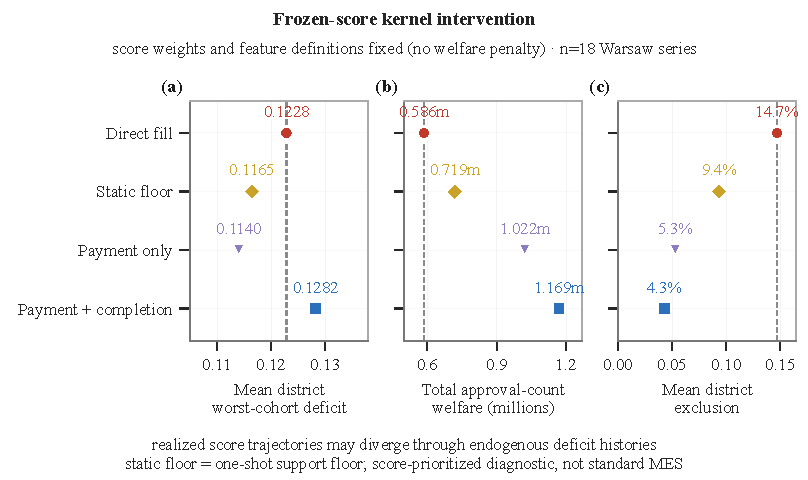
\includegraphics[width=0.98\textwidth]{fig_hack.pdf}
\caption{Frozen-score allocation-kernel intervention on
$n=\EvalSeriesN{}$ Warsaw district series. The panels compare mean worst-group
CSD, total approval-count welfare, and mean exclusion under
direct fill, a one-shot support floor, score-prioritized approver-funded
payment, and payment plus completion. Score weights and feature definitions
remain fixed. Realized score trajectories may still diverge because each rule
generates its own deficit history. Payment plus completion lowers exclusion
from \KernelDirectExcl{} to \KernelPaymentCompleteExcl{} and multiplies welfare
by \KernelPaymentCompleteWelfareFactor$\times$; the CSD change is not detectable
($p$~\KernelPaymentCompleteCSDP). The diagnostic is not standard \MES{} and
provides neither a universal nor an external guarantee.}
\label{fig:hack}
\end{figure}

The following tables use the same result files as the main text. They report
the values for each series, seed, partition, and condition that underlie the
aggregates.

\begin{table}[tb]
\centering\small
\begin{tabular}{lccc}
\toprule
Condition (no welfare penalty) & Mean worst-group $\csd$ & Welfare & Exclusion \\
\midrule
Outcome family, unconstrained & \LearnedCornerCSD & \LearnedCornerWelfare & \LearnedCornerExcl \\
\quad + support floor $\kappa = 1$ & \IdentKOneCSD & \IdentKOneWelfare & \IdentKOneExcl \\
\quad + support floor $\kappa = 2$ & \IdentKTwoCSD & \IdentKTwoWelfare & \IdentKTwoExcl \\
\midrule
Learned endowment map (reference) & \EndowCSD & \EndowWelfare & \EndowExcl \\
\MES{} (reference) & \TestMESCSD & \TestMESWelfare & \TestMESExcl \\
\bottomrule
\end{tabular}
\caption{Retrained static-floor control for Proposition~\ref{prop:support}. We
fit the outcome family with \emph{no welfare penalty}. The support floor adds
a one-shot coverage restriction without iterative approver payment.
At $\kappa=1$, all three reported outcomes improve over the unconstrained
policy, yet welfare remains roughly forty percent below Equal Shares and
exclusion roughly twice as high. Table~\ref{tab:kernel-intervention} instead
holds the learned score weights fixed and introduces payment dynamics
separately.}
\label{tab:identification}
\end{table}

\label{app:tables}

\begin{table}[t]
\centering\small
\begin{tabular}{lccccc}
\toprule
& Welfare target $\tau$ & Worst $\csd$ & Mean $\csd$ & Welfare & Exclusion \\
\midrule
\multicolumn{6}{l}{\emph{Endowment family (mechanism retained)}}\\
& 0.00 & 0.1743 & 0.0374 & 1,274,522 & 0.0418 \\
& 0.99 & 0.1736 & 0.0371 & 1,277,125 & 0.0418 \\
& 1.00 & 0.1876 & 0.0395 & 1,284,042 & 0.0433 \\
\midrule
\multicolumn{6}{l}{\emph{Outcome family (mechanism discarded)}}\\
& 0.00 & 0.1228 & 0.0024 & 586,114 & 0.1470 \\
& 0.85 & 0.1153 & 0.0101 & 1,198,311 & 0.0450 \\
& 0.95 & 0.1483 & 0.0228 & 1,259,890 & 0.0442 \\
& 1.00 & 0.1728 & 0.0320 & 1,303,057 & 0.0447 \\
& 1.02 & 0.1828 & 0.0352 & 1,310,536 & 0.0451 \\
& 1.05 & 0.1869 & 0.0364 & 1,312,691 & 0.0450 \\
\bottomrule
\end{tabular}
\caption{Sweeps over soft welfare targets for both arms at seed 42 on held-out Warsaw districts. Worst $\csd$ is the equal-weight mean district-level worst-group value; lower CSD and exclusion and higher welfare are favorable. Targets are penalties, not hard constraints. This single-seed descriptive sweep has no intervals; corpus- and budget-specific ranges are not universal reachable sets.}
\label{tab:endowfrontier}
\end{table}

